Приёмники света (глаз человека, фотопластинка, фотоэлемент) реагируют на поток энергии световой 
волны, т. е. величину, пропорциональную квадрату амплитуды. Информация о фазовой структуре волны 
(т. е. о форме волнового фронта) оказывается при этом утраченной.

В этом разделе мы рассмотрим способ записи изображения, который позволяет по картине интенсивности 
восстановить полную информацию о волновом поле.

\begin{wrapfigure}{r}{0.4\linewidth}
  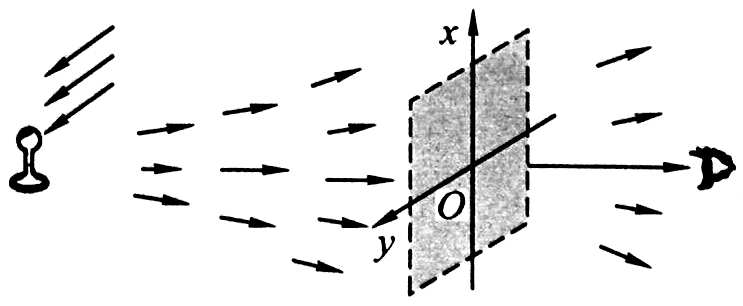
\includegraphics[width=\linewidth]{3.47.png}
  \caption{Световое поле предмета}
  \label{img::3_47}
\end{wrapfigure}

Пусть некоторый предмет (пешка, изображённая на рис. (\ref{img::3_47})) освещается когерентным светом
лазера и пусть волна, отражённая предметом (будем называть её далее предметной волной), создаёт в
плоскости $z = 0$ световое поле:

$$
f_{\text{П}}(x, y) = a(x, y) \cdot \e^{i \varphi(x, y)}
$$

Установим в плоскости $z = 0$ фотопластинку. Предположим, что функция пропускания фотопластинки 
после необходимой обработки (проявление, закрепление) пропорциональна интенсивности волны,
освещающей пластину во время экспозиции, т. е. пропорциональна величине $I(x, y) = |a(x, y)|^2$.
Информация о фазовой структуре волны $\varphi(x, y)$ будет при этом утеряна.

\begin{wrapfigure}{r}{0.35\linewidth}
  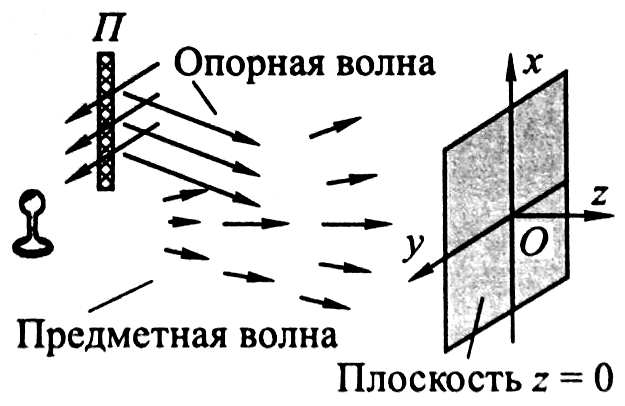
\includegraphics[width=\linewidth]{3.48.png}
  \caption{Запись голограммы}
  \label{img::3_48}
\end{wrapfigure}

Следуя идее Габора (1948 г.), изменим схему эксперимента: пусть на фотопластинку кроме предметной 
волны, создающей на фотопластинке поле $f_{\text{п}}(x, y)$ , падает ещё некоторая волна с известным 
распределением амплитуд и фаз колебаний $f_o(x,y) = a_o(x, y) \e^{i \varphi(x, y)}$ , называемая 
опорной волной (см. рис. \ref{img::3_48}). При этом необходимо обеспечить когерентность предметной и 
опорной волны -- волны должны интерферировать. Например, как показано на рис. \ref{img::3_48}:
излучение лазера частично проходит через полупрозрачную пластинку $\text{П}$, освещая предмет, а 
частично отражается от неё, создавая опорный пучок. Когерентность предметной и опорной волн 
обеспечивается высокой степенью монохроматичности лазерного излучения (разность хода между предметной
и опорной волнами меньше длины когерентности для любой точки фотопластинки).

Суммарное поле на голограмме

$$
f(x,y) = f_{\text{п}}(x, y) + f_o(x,y)
$$
\\
а интенсивность (а следовательно, и функция пропускания фотопластинки после необходимой обработки) 
есть

$$
t(x,y) \propto I(x, y) = |f_{\text{п}}(x, y) + f_o(x,y)|^2
$$
\\
Раскрывая квадрат модуля в полученном выражении

$$
t \propto |f_{\text{п}}|^2 + |f_o(x,y)|^2 + f_{\text{п}} f_o^* + f_{\text{п}}^* f_o =
          a^2 + a_o^2 + 2 a a_o \cos (\varphi - \varphi_o)
$$
\\
убеждаемся, что в функции пропускания (а именно, в слагаемом, связанном с интерференцией опорной
и предметной волн) сохранилась информация о фазе предметной волны $\varphi(x, y)$

Фотопластинка с зарегистрированным на ней результатом интерференции предметной и опорной волны 
называются голограммой.